\chapter{Projektive Geometrie}
\section{Hessesche Normalform}
\subsection{der Gerade}
Die Gleichung \begin{displaymath} \frac{Ax + By + C}{\sqrt{A^{2} + B^{2}}} = 0 \end{displaymath} heisst hessische Normalform der \textbf{Gerade}. \\
Wird die Gleichung erfüllt, liegt der Punkt auf der Geraden, andernfalls resultiert der Abstand  zur Geraden (inkl. auf welcher Seite).
\subsubsection{Definition}
Die Gleichung wird genau von den Punkten erfüllt, die auf der Geraden (welche die Gleichung beschreibt)
liegen. Liegt der Punkt nicht auf der Geraden, so liefert die Hesse’sche Normalenform den Abstand vom Punkt
zur Geraden. Das Vorzeichen gibt an, ob der Punkt auf der Seite der Geraden liegt, in deren Richtung der
Normalenvektor zeigt, oder ob er auf der anderen Seite der Geraden liegt.

\subsubsection{Beispiel Geradengleichung}
Wir betrachten die Geradengleichung \begin{displaymath} 3x + y - 5 = 0 \end{displaymath} und bestimmen die HN:
\begin{displaymath} \frac{3x+y-5}{\sqrt{3^{2} + 1^{2}}} \text{ resp. } \frac{3x+y-5}{\sqrt{10}} \end{displaymath}
Wir testen die folgenden Punkte \begin{displaymath}S(3;-4)\\T(2; -5)\\ U(2; 5) \end{displaymath}
Der Punkt \(S\) in die HN eingesetzt ergibt: \begin{displaymath} \frac{3\cdot3 + (-4) -5}{\sqrt{10}} = \frac{9-9}{\sqrt{10}} = 0 \end{displaymath}, somit liegt \(S\) auf der Geraden.\\
Der Punkt \(T\) in die HN eingesetzt ergibt: \begin{displaymath}\frac{3\cdot2 + (-5) -5}{\sqrt{10}} = \frac{6-10}{\sqrt{10}} = -1.265 \end{displaymath}, somit liegt \(T\) nicht auf der Geraden. Der Punkt \(T\) hat einen Abstand von 1,256 LE von der Gerade und liegt dem Normalenvektor entgegengesetzt. \\
Der Punkt \(U\) in die HN eingesetzt ergibt: \begin{displaymath} \frac{3\cdot2 +5-5}{\sqrt{10}} = \frac{6}{\sqrt{10}} = 1.897 \end{displaymath}, somit liegt \(U\) nicht auf der Geraden. Der Punkt \(U\) hat einen Abstand von 1,897 LE von der Gerade und liegt auf der „positiven“ Seite der Geraden.
\subsection{zur Ebene}
Die Gleichung \begin{displaymath} \frac{Ax + By + Cz + D}{\sqrt{A^{2} + B^{2} + C^{2}}} = 0 \end{displaymath} heisst hessische Normalform der \textbf{Ebene}.
\subsubsection{Definition}
\begin{itemize}
    \item Ergibt das Einsetzten eines Punktes in der HN \(= 0\), so liegt der Punkt in der Ebene.
    \item Ergibt das Einsetzten eines Punktes in der HN \(d > 0\), so liegt der Punkt auf der gleichen Seite des Normalenvektors \( \vec{n_{E}}= \begin{pmatrix} A \\ B \\ C \end{pmatrix} \) mit Abstand \(d\) zur Ebene. 
    \item Ergibt das Einsetzten eines Punktes in der HN \(d < 0\), so liegt der Punkt auf der entgegengesetzten Seite des Normalenvektors \(\vec{n_{E}} = \begin{pmatrix} A \\ B \\ C \end{pmatrix} \) mit Abstand \(|d|\) zur Ebene.
\end{itemize}
\subsubsection{Beispiel}
Gegeben ist die Koordinatengleichung der Ebene E: \(x - 4 \cdot y + 2 \cdot z + 9 = 0 \)\\
Gesucht der Abstand der Punkte \(Q(3; -1; -4)\text{, }R(5; 6; -7) \text{ und } S(3; 7; 8)\) zur Ebene.
\begin{description} 
    \item[1. Schritt: Bestimmen der HN der Ebene]
    \begin{displaymath}
    \text{HN: } \frac{Ax + By + Cz + D}{\sqrt{A^{2} + B^{2} + C^{2}}} = \frac{x - 4\cdot y + 2 \cdot z + 9}{\sqrt{1^{2} + (-4)^{2} + 2^{2}}} = \frac{x - 4 \cdot y + 2 \cdot z + 9}{\sqrt{21}} = 0
    \end{displaymath}
    \item[2. Schritt: Einsetzten der Punkte:]
    \(\text{ }\\ Q(3; -1; -4): \)
    \begin{displaymath}
   \frac{x - 4 \cdot y + 2 \cdot z + 9}{\sqrt{21}} = \frac{3 - 4 \cdot (-1) + 2 \cdot (-4) + 9}{\sqrt{21}} = \frac{8}{\sqrt{21}} = 1.746
   \end{displaymath}
   Der Punkt liegt also dem Normalenvektor \( \vec{n_{E}} = \begin{pmatrix} 1 \\ -4 \\ 2 \end{pmatrix} \) gleich gesetzten Seite der Ebene mit dem Abstand 1.746 LE zur Ebene.\\
    \(\text{ }\\R(5; 6; -7):\\ \)
    \begin{displaymath}
    \frac{5 - 4 \cdot 6 + 2 \cdot (-7) + 9}{\sqrt{21}} = \frac{-24}{\sqrt{21}} = -5.237
    \end{displaymath}
    Der Punkt liegt also dem Normalenvektor \( \vec{n_{E}} \) entgegengesetzte Seite der Ebene mit dem Abstand 5.237 LE zur Ebene.\\
    \(\text{ }\\S(3; 7; 8): \\ \)
    \begin{displaymath}
    \frac{3 - 4 \cdot 7 + 2 \cdot 8 + 9}{\sqrt{21}} = \frac{0}{\sqrt{21}} = 0\\
   \end{displaymath}
   Der Punkt liegt auf der Ebene (es ist ja auch unser ursprünglicher Punkt C.)
\end{description}


\section{Skalare und Vektoren und das Kartesisches Koordinatensystem}

\begin{description}
	\item[Skalar]
	ist eine reelle (oder komplexe) Zahl. Beispiele: Temperatur,
	Druck, Luftfeuchtigkeit.
	\item[Vektor]
	hat einen (reellen) Betrag und eine Richtung. Beispiele:
	(Wind-) Geschwindigkeit (an einem Ort), Kraft (auf ein
	Objekt), Fliessgeschwindigkeit in Gewässern, Elektrisches
	Feld, Magnetfeld, Gravitationsfeld, etc.
\end{description}

\subsection{Addition von Vektoren und Multiplikation mit einem Skalar}

Gegeben sind die Vektoren:
\begin{math}
	\vec{a} = 
	\begin{pmatrix} a_{1} \\ a_{2} \end{pmatrix}
\end{math}
und
\begin{math}
	\vec{b} = 
	\begin{pmatrix} b_{1} \\ b_{2} \end{pmatrix}
\end{math}

\begin{description}
	\item[Addition:]
	Zwei Vektoren $\vec{a}$ und $\vec{b}$ addieren heisst entsprechende Komponenten addieren. 
\end{description}

\begin{math}
	\vec{a} + \vec{b} = 
	\begin{pmatrix} a_{1} \\ a_{2} \end{pmatrix} +
	\begin{pmatrix} b_{1} \\ b_{2} \end{pmatrix} =
	\begin{pmatrix} a_{1} + b_{1} \\ a_{2} + b_{2} \end{pmatrix}
\end{math}

\begin{description}
	\item[Multiplikation mit Skalar:]
	Einen Vektor $\vec{a}$ mit einem Skalar $\lambda \in \mathbb{R}$ multiplizieren. 
\end{description}

\begin{math}
	\lambda \vec{a} = 
	\lambda \begin{pmatrix} a_{1} \\ a_{2} \end{pmatrix} =
	\begin{pmatrix} \lambda a_{1} \\ \lambda a_{2} \end{pmatrix}
\end{math}

\subsection{Das Inverse eines Vektors und der Nullvektor}

\begin{description}
	\item[Inverse:]
	Das Inverse $-\vec{a}$ des Vektors
	\begin{math}
		\vec{a} = \begin{pmatrix} a_{1} \\ a_{2} \end{pmatrix}
	\end{math}
	ist der Vektor mit den negativen Komponenten:
	\begin{math}
		-\vec{a} = -\begin{pmatrix} a_{1} \\ a_{2} \end{pmatrix} =
		\begin{pmatrix} -a_{1} \\ -a_{2} \end{pmatrix}
	\end{math}
\end{description}

\begin{description}
	\item[Nullvektor:]
	Der Nullvektor $\vec{0}$ ist ein Vektor dessen Komponenten alle
	verschwinden (also gleich Null sind):
	\begin{math}
		\vec{0} = \begin{pmatrix} 0 \\ 0 \end{pmatrix}
	\end{math}
\end{description}

Damit wird die Subtraktion des Vektors $\vec{b}$ vom Vektor $\vec{b}$ wie folgt definiert:
\begin{math}
	\vec{a} -\vec{b} = \vec{a} + \begin{pmatrix} -\vec{b} \end{pmatrix}
\end{math}

\begin{description}
	\item[Rechenregeln:]
\end{description}
\begin{math}
	\vec{a} + \vec{b} = \vec{b} + \vec{a}
\end{math}
Kommutativgesetz\\
\begin{math}
	\vec{a} + (\vec{b} + \vec{c}) = (\vec{a} + \vec{b}) + \vec{c}
\end{math}
Assoziativgesetz\\
\begin{math}
	\vec{a} + 0 = \vec{a}
\end{math}
Existenz eines Neutralelements $\vec{0}$\\
$\vec{a} + \vec{-a} = \vec{0}$\\
$\lambda (\vec{a} + \vec{b}) = \lambda \vec{a} + \lambda \vec{b}$\\
$(\lambda + \mu) \vec{a} = \lambda \vec{a} + \mu \vec{a}$\\
$(\lambda \mu) \vec{a} = \lambda (\mu \vec{a}) = \mu (\lambda \vec{a})$
\newpage

\subsection{Geometrische Interpretation}

Zwei Vektoren sind gleich, wenn ihre Komponenten gleich sind!
Achtung: In der Physik darf man z.B. Kraftvektoren nicht einfach
verschieben!

\begin{figure}[!ht]
	\centering
	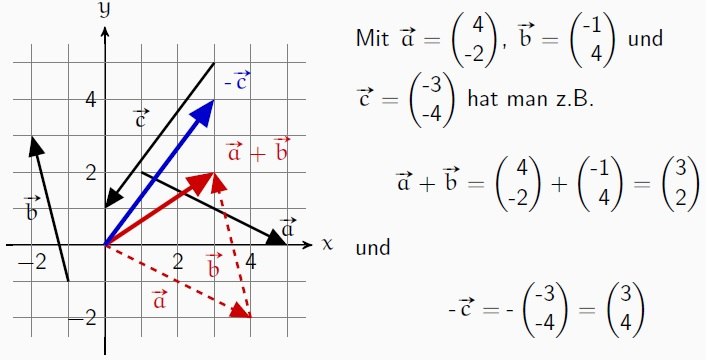
\includegraphics[width=0.7\linewidth]{fig/geometrische_interpretation}
	\caption{Geometrische Interpretation}
	\label{fig:geometrische_interpretation}
\end{figure}

Es folgt nun ein Example zur Berechnung von Vektoren.
Bestimmen Sie
\begin{math}
	3 \vec{a} - 2 \vec{b} + \vec{c}
\end{math}
sowohl grafisch wie auch rechnerisch (analytisch). Details der Vektoren sind in Abbildung \ref{fig:geometrische_interpretation} zu entnehmen.

\begin{math}
	3 \begin{pmatrix} 4 \\ -2 \end{pmatrix} - 
	2 \begin{pmatrix} -1 \\ 4 \end{pmatrix} + 
	\begin{pmatrix} -3 \\ -4 \end{pmatrix} = 
	\begin{pmatrix} 12 \\ -6 \end{pmatrix} -
	\begin{pmatrix} -2 \\ 8 \end{pmatrix} +
	\begin{pmatrix} -3 \\ -4 \end{pmatrix} =
	\begin{pmatrix} 11 \\ -18 \end{pmatrix}
\end{math}

\begin{description}
	\item[Basisvektoren:]
	Die Basisvektoren $\vec{e}_x$ und $\vec{e}_y$ sind orthogonal und haben die Länge 1,\\
	d.h. $\vec{e}_x \cdot \vec{e}_x = 0$ und $\mid \vec{e}_x \mid = 1$ sowie $\mid \vec{e}_y \mid = 1$.
\end{description}

\section{Skalarprodukt}

Das Skalarprodukt zweier Vektoren $\vec{a}$ und $\vec{b}$ ist wie folgt definiert:\\
$\vec{a} \cdot \vec{b} = \mid \vec{a} \mid \dot \mid \vec{b} \mid cos(\phi)$\\
In kartesischen Koordinaten gilt:\\
$\vec{a} \cdot \vec{b} =
\begin{pmatrix} a_{1} \\ a_{2} \end{pmatrix} \cdot
\begin{pmatrix} b_{1} \\ b_{2} \end{pmatrix} =
a_{1} b_{1} + a_{2} b_{2}$

Es folgt ein Beispiel dazu:\\
Gegeben sind die Vektoren 
$\vec{a} = \begin{pmatrix} 4 \\ -2 \end{pmatrix}$
und
$\vec{b} = \begin{pmatrix} -1 \\ 4 \end{pmatrix}$
man berechne nun das Skalarprodukt sowie den Winkel $\phi$.\\

\begin{math}
	\vec{a} \cdot \vec{b} = 
	\begin{pmatrix} 4 \\ -2 \end{pmatrix} + 
	\begin{pmatrix} -1 \\ 4 \end{pmatrix} =
	4 (-2) + (-1) 4 = -4 -8 = -12
\end{math}

\begin{math}
	a = \mid \vec{a} \mid = 
	\sqrt{\vec{a_{1}^2} + \vec{a_{2}^2}} =
	\sqrt{4^2 + (-2)^2} =
	\sqrt{20}
\end{math}

\begin{math}
	b = \mid \vec{b} \mid = 
	\sqrt{\vec{b_{1}^2} + \vec{b_{2}^2}} =
	\sqrt{(-1)^2 + 4^2} =
	\sqrt{17}
\end{math}

\begin{math}
	cos(\phi) =
	\frac{\vec{a} \cdot \vec{b}}{\mid \vec{a} \mid \dot \mid \vec{b} \mid} = 
	\frac{-12}{\sqrt{20} \sqrt{17}} = 
	-0.6508
\end{math}
\\Daraus folgt mit $\arccos(\phi)$:
\begin{math}
	\phi = \arccos(-0.6508) = 130.6^\circ
\end{math}
\\$\mid \vec{a} \mid$ ist die Länge des Vectors $\vec{a}$.

\begin{description}
	\item[Rechengesetze]
\end{description}
$\vec{a} \cdot \vec{b} = \vec{b} \cdot \vec{a}$ Kommutativgesetz\\
$\vec{a} \cdot (\vec{b} + \vec{c}) = 
\vec{a} \cdot \vec{b} + \vec{a} \cdot \vec{c}$
Distributivgesetz\\
$\lambda (\vec{a} \cdot \vec{b}) = 
(\lambda \vec{a}) \cdot \vec{b} = 
\vec{a} \cdot (\lambda \vec{b})$

\begin{description}
	\item[Orthogonale Vektoren]
	Zwei Vektoren $\vec{a}$ und $\vec{b}$ stehen genau dann senkrecht aufeinander, sind also orthogonal, falls ihr Skalarprodukt verschwindet respektive 0 ist.\\
	\begin{math}
		\vec{a} \cdot \vec{b} = 0 \iff \vec{a} \perp \vec{b}
	\end{math}
	\\Angenommen ein der Vektor $\vec{a} = \begin{pmatrix} 2 \\ 1 \end{pmatrix}$ sei gegeben. Um einen dazugehörenden orthogonalen Vektor zu erhalten muss folgende Formel aufgelöst werden:\\
	\begin{math}
		2b_{1} + 1b_2 = 0
	\end{math}
	\\Ein möglicher Vektor wäre also $\vec{b} = \begin{pmatrix} -1 \\ 2 \end{pmatrix}$ oder ein Vielfaches davon!
\end{description}
\section{Spatprodukt}

Das Spatprodukt $[\vec{a}, \vec{b}, \vec{c}]$ der drei Vektoren $\vec{a}$, $\vec{b}$ und $\vec{c}$ ist das Skalar $[\vec{a}, \vec{b}, \vec{c}] = \vec{a} \cdot (\vec{b} \times \vec{c})$.
Der Betrag des Spatprodukts $\mid [\vec{a}, \vec{b}, \vec{c}] \mid$ ist das Volumen des durch die drei Vektoren $\vec{a}$, $\vec{b}$ und $\vec{c}$ aufgespannten Spats.

\begin{figure}[!ht]
	\centering
	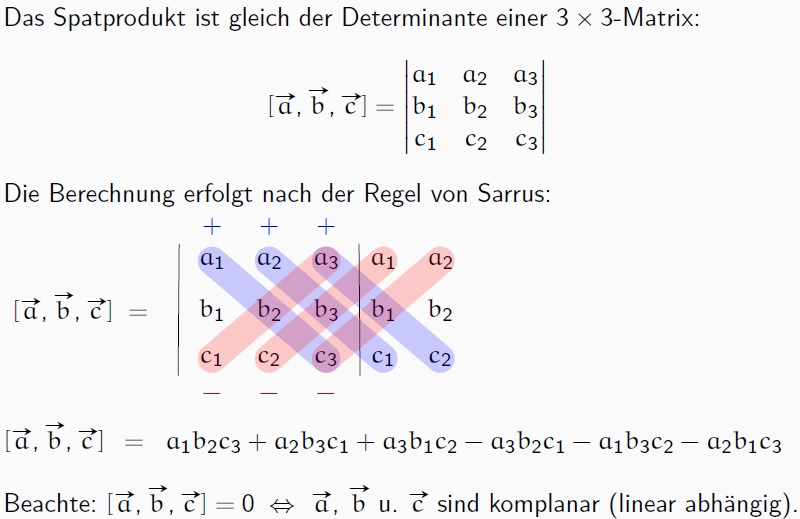
\includegraphics[width=0.7\linewidth]{fig/spatprodukt}
	\caption{Spatprodukt}
	\label{fig:spatprodukt}
\end{figure}

\begin{description}
	\item[Rechenregeln für das Spatprodukt]
\end{description}
Vertauschen von zwei Vektoren bewirkt einen Vorzeichenwechsel: z.B.\\
$[\vec{a}, \vec{b}, \vec{c}]$ = $-[\vec{b}, \vec{a}, \vec{c}]$\\
Zyklisches Vertauschen der drei Vektoren ändert nichts:\\
$[\vec{a}, \vec{b}, \vec{c}] = [\vec{b}, \vec{c}, \vec{a}] = [\vec{c}, \vec{a}, \vec{b}]$\\
Multiplikation der Vektoren mit reellen Zahlen $\lambda$, $\mu$, $\nu$:\\
$[\lambda \vec{a}, \mu \vec{b}, \nu \vec{c}] = \lambda \mu \nu [\vec{a}, \vec{b}, \vec{c}]$\\
Addition zweier Vektoren\\
$[\vec{a} + \vec{b}, \vec{c}, \vec{d}] = [\vec{a}, \vec{c}, \vec{d}] + [\vec{b}, \vec{c}, \vec{d}]$

\section{Transformation: Translation in 2D}
Um eine Figur in eine Richtung zu verschieben, kann man alle ihre Punkte als Matrix zusammennehmen, diese in eine höhere Dimension nehmen (in homogene Koordinaten umschreiben) und die Translation in derselben Dimension vornehmen, indem man in der rechtesten Spalte der Einheitsmatrix die Verschiebungen vornimmt.

\subsection{Beispiel Translation 2D}

Gegeben sind die Punkte $A=(3,1)$, $B=(6,1)$ und $C=(5,4)$ und die Verschiebungsrichtung $\vec{t} = \begin{pmatrix}1 & 2
\end{pmatrix}$. 

Man nimmt nun die Punkte alle zusammen in einer Matrix und erweitert diese die homogenen Koordinaten mit dem Wert 1 in der dritten Dimension (dargestellt unterhalb des Strichs in der Matrix):

\[
Points = \begin{pmatrix}
A_x & B_x & C_x\\
A_y & B_y & C_y\\ \hline
1 & 1 & 1
\end{pmatrix} = \begin{pmatrix}
3 & 6 & 5\\
1 & 1 & 4\\ \hline
1 & 1 & 1
\end{pmatrix}
\]

Den Verschiebungsvektor macht man nun zur Matrix. Dazu wird die Einheitsmatrix der neuen homogenen Dimension genommen und als rechteste Spalte wird der Vektor $\vec{t}$ eingesetzt. $\vec{t}$ wird als zu 

$T=\begin{pmatrix}
1 & 0 & t_x\\
0 & 1 & t_y\\
0 & 0 & 1
\end{pmatrix}=\begin{pmatrix}
1 & 0 & 1\\
0 & 1 & 2\\
0 & 0 & 1
\end{pmatrix}$

Nun muss man nur noch $T \cdot  M$ berechnen:
\begin{align}
\begin{split}
T\cdot Points &=\begin{pmatrix}
1 & 0 & 1\\
0 & 1 & 2\\
0 & 0 & 1
\end{pmatrix} \cdot  \begin{pmatrix}
3 & 6 & 5\\
1 & 1 & 4\\
1 & 1 & 1
\end{pmatrix}\\
&= \begin{pmatrix}
A_x' & B_x' & C_x'\\
A_y' & B_y' & C_y'\\ \hline
1 & 1 & 1
\end{pmatrix} = \begin{pmatrix}
4 & 7 & 6\\
3 & 3 & 6\\ \hline
1 & 1 & 1
\end{pmatrix}
\end{split}
\end{align}

Die Punkte der neuen Koordinaten sind also $A'=(4,3)$, $B'=(7,3)$ und $C'=(6,6)$.

\section{Transformation: Rotation um einen Winkel $\Phi$ in 2D}

Die Rotation um wird vorgenommen, indem folgende Matrix verwendet wird:
\[
T = \begin{pmatrix}
\cos (\Phi) & -\sin (\Phi) & 0\\
\sin (\Phi) & \cos (\Phi) & 0\\
0 & 0 & 1
\end{pmatrix}
\]

\section{Transformation: Rotation in 3D}

\subsection{Rotation einen Winkel $\Phi$ um die z-Achse}

$\textbf{R}_z(\Phi_z) = \begin{pmatrix}
\cos (\Phi) & -\sin (\Phi) & 0 & 0\\
\sin (\Phi) & \cos (\Phi) & 0 & 0\\
0 & 0 & 1 & 0\\
0 & 0 & 0 & 1
\end{pmatrix}$

Inverse davon ist:
$\textbf{R}_z^{-1}(\Phi_z) = \begin{pmatrix}
\cos (\Phi) & \sin (\Phi) & 0 & 0\\
-\sin (\Phi) & \cos (\Phi) & 0 & 0\\
0 & 0 & 1 & 0\\
0 & 0 & 0 & 1
\end{pmatrix}$

\subsection{Rotation einen Winkel $\Phi$ um die y-Achse}

$\textbf{R}_y(\Phi_y) = \begin{pmatrix}
\cos (\Phi) & 0 & \sin (\Phi) & 0\\
0 & 1 & 0 & 0\\
-\sin (\Phi) & 0 & \cos (\Phi) & 0\\
0 & 0 & 0 & 1
\end{pmatrix}$

Inverse davon ist:
$\textbf{R}_y^{-1}(\Phi_y) = \begin{pmatrix}
\cos (\Phi) & 0 & -\sin (\Phi) & 0\\
0 & 1 & 0 & 0\\
\sin (\Phi) & 0 & \cos (\Phi) & 0\\
0 & 0 & 0 & 1
\end{pmatrix}$

\subsection{Rotation einen Winkel $\Phi$ um die x-Achse}

$\textbf{R}_x(\Phi_x) = \begin{pmatrix}
1 & 1 & 0 & 0\\
0 & \cos (\Phi)  & -\sin (\Phi) & 0\\
0 & \sin (\Phi) & \cos (\Phi) & 0\\
0 & 0 & 0 & 1
\end{pmatrix}$

Inverse davon ist:
$\textbf{R}_x^{-1}(\Phi_x) = \begin{pmatrix}
1 & 1 & 0 & 0\\
0 & \cos (\Phi)  & \sin (\Phi) & 0\\
0 & -\sin (\Phi) & \cos (\Phi) & 0\\
0 & 0 & 0 & 1
\end{pmatrix}$

\subsection{Rotation um eine beliebige Achse}
\begin{enumerate}
\item Rotation um den Winkel $\Phi$ um die z-Achse (hier Matrix D genannt)
\item Rotation um den Winkel $\Theta$ um die frühere x-Achse mit der Matrix C.
\item Rotation um den Winkel $\Psi$ um die frühere z-Achse mit der Matrix B.
\end{enumerate}

Man hat nun die Matrizen:
\begin{figure}[!ht]
	\centering
	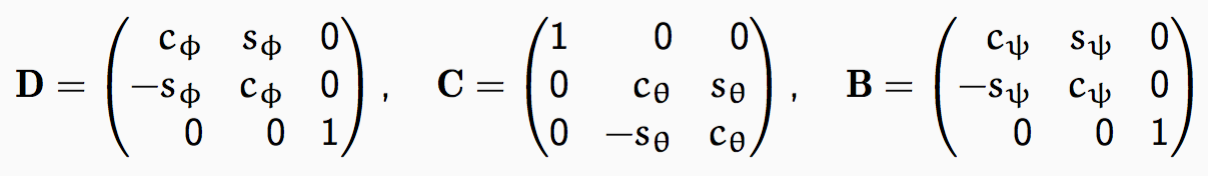
\includegraphics[width=0.7\linewidth]{fig/Rotation_um_bel_Achse.png}
	\caption{Rotationsmatrizen}
	\label{fig:spatprodukt}
\end{figure}

Diese kann man als eine Transformation zusammennehmen durch Multiplikation:
\begin{figure}[!ht]
	\centering
	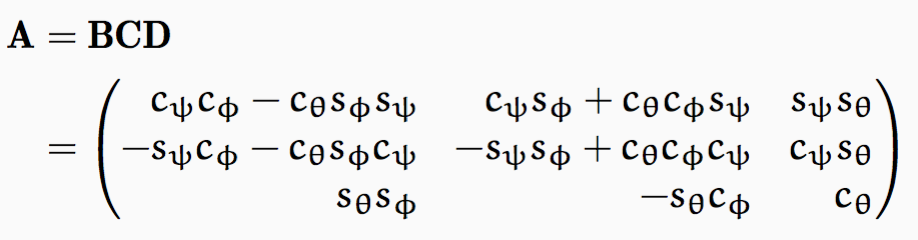
\includegraphics[width=0.7\linewidth]{fig/Zusammengesetzte_Rotationsmatrix.png}
	\caption{Zusammengesetzte Rotationsmatrix}
	\label{fig:spatprodukt}
\end{figure}

\newpage

\section{Transformation: Spiegelung an einer Geraden}
Eine direkte Spiegelung ist nur möglich, wenn die Gerade durch den Ursprung geht. Tut sie dies nicht, muss zuerst eine Translation durchgeführt werden. Dies macht man folgendermassen.

Einer Geraden $g$ sieht man gleich zu Beginn an, ob sie durch den Nullpunkt geht, nämlich wenn sie eine Verschiebungskonstante hat, also in der Form $g = ax + by + c$ mit $c \neq 0$ vorliegt.

Nach der Verschiebung findet die eigentliche Spiegelung statt. Dazu muss man zuerst herausfinden, in welchem Winkel die Gerade zum Ursprung steht. Dazu verwendet man den Tangens, weil bekannt ist, in welchem Verhältnis $x$ zu $y$ steht, nämlich mit der Steigung $m$ (vergleiche dazu die Gleichung $y = mx + q$)! Man kann also den Arcus-Tangens verwenden, um $\delta$ herauszufinden:

\begin{align}
\begin{split}
\tan (\delta) &= m \\
\delta &= \arctan (m)
\end{split}
\end{align}

Man könnte auch direkt in Kosinus und Sinus umwandeln mit der Formel:

\begin{align}
\begin{split}
\cos (2\delta) &= \frac{1-\tan^2 (\delta)}{1+\tan^2 (\delta)}\\
\sin (2\delta) &= \frac{2\tan^2 (\delta)}{1+\tan^2 (\delta)}
\end{split}
\end{align}

Danach verwendet man die \textbf{Nullpunkt-Spiegelungsmatrix}:

\[
\sigma' =\begin{pmatrix}
\cos (2\delta) & \sin (2\delta) & 0\\
\sin (2\delta) & -\cos (2\delta) & 0\\
0 & 0 & 1\\
\end{pmatrix}
\]

Jetzt muss man nur noch die Translation rückgängig machen mit $T^{-1}$ (Inverse von T).

Zusammengesetzt ergibt sich die \textbf{Spiegelungsmatrix} $\sigma = T^{-1}*\sigma'*T$.\\

Die \textbf{Bildpunkte} erhält man durch Multiplikation der Punkte mit der Spiegelungsmatrix:
\[
A' = \sigma * A
\]

\subsection{Beispiel}
Gegeben ist die Gerade $g = 2x - 3y + 2$. Wir wollen die Spiegelung $\sigma$ an dieser Geraden betrachten. Gesucht sind:

\begin{enumerate}
\item \textbf{Die Matrix $\sigma$}

Man bringt die Gerade erstmal in die Form $y = mx + q$:
\begin{align}
\begin{split}
2x - 3y + 2 &= 0\\
\Rightarrow y &= \frac{2x + 2}{3}
\end{split}
\end{align}
Um nun einen Punkt der Geraden zu finden, muss man einfach für $x$ einsetzen (ich wähle 2, da es so eine schöne Lösung gibt):
\begin{align}
\begin{split}
y &= \frac{2*2 + 2}{3}\\
&=  \frac{6}{3} = 2
\end{split}
\end{align}
Ein Punkt, der auf der Geraden liegt, ist also $p_g = (2,2)$.

Das heisst, dass die Translationsmatrix folgendermassen aussieht (so wird der Punkt in den Ursprung verschoben):
\[
T_{p_g} = \begin{pmatrix}
1 & 0 & -2\\
0 & 1 & -2\\
0 & 0 & 1
\end{pmatrix}
\]

Wir kennen das Verhältnis von der Gegenkatete zur Ankatete, nämlich: 

\[
\tan (\delta) = \frac{2}{3}
\]

Eingesetzt können wir nun berechnen:
\begin{align}
\begin{split}
\cos (2\delta) = \frac{1-\frac{2}{3}^2}{1+\frac{2}{3}^2} = \frac{1-\frac{4}{9}}{1+\frac{4}{9}} = \frac{\frac{5}{9}}{\frac{13}{9}} &= \frac{5}{13}\\
\sin (2\delta) = \frac{2\frac{2}{3}}{1+\frac{2}{3}^2} = \frac{\frac{4}{3}}{1+\frac{4}{9}} = \frac{\frac{12}{9}}{\frac{13}{9}} = \frac{12}{13} &= \frac{12}{13}\\
\end{split}
\end{align}

Nun muss man dies nur noch in die Spiegelungsmatrix einsetzen:

\[
\sigma' = 
\begin{pmatrix}
\frac{5}{13} & \frac{12}{13} & 0\\
\frac{12}{13} & -\frac{5}{13} & 0\\
0 & 0 & 1
\end{pmatrix}
\]

Schliesslich kann man "da real"-Spiegelungsmatrix $\sigma$ folgendermassen berechnen:

\[
\underline{\underline{\sigma = T^{-1}\sigma T = 
\begin{pmatrix}
\frac{5}{13} & \frac{12}{13} & -\frac{8}{13}\\
\frac{12}{13} & -\frac{5}{13} & \frac{12}{13}\\
0 & 0 & 1
\end{pmatrix}}}
\]

\item Die Bildpunkte von $A = (8, 1)$ und $B=(-65.4, 0.2)$.

Man setzt die Punkte in die Matrix:

\[
Points = \begin{pmatrix}
8 & -65.4 \\
1 & 0.2 \\
1 & 1
\end{pmatrix}
\]

Danach berechnet man $\sigma * Points$ und erhält das Resultat:

\[
ResultMatrix = \begin{pmatrix}
3.38... & -25.58... \\
7.92... & -59.52... \\
1 & 1
\end{pmatrix}\textnormal{, } 
\underline{\underline{A' = 
\begin{pmatrix}
3.38...\\
7.92... 
\end{pmatrix}\textnormal{, } 
B' = 
\begin{pmatrix}
-25.58... \\
-59.52... 
\end{pmatrix}}}
\]

\end{enumerate}

\section{Vektorprodukt}

\begin{figure}[!ht]
	\centering
	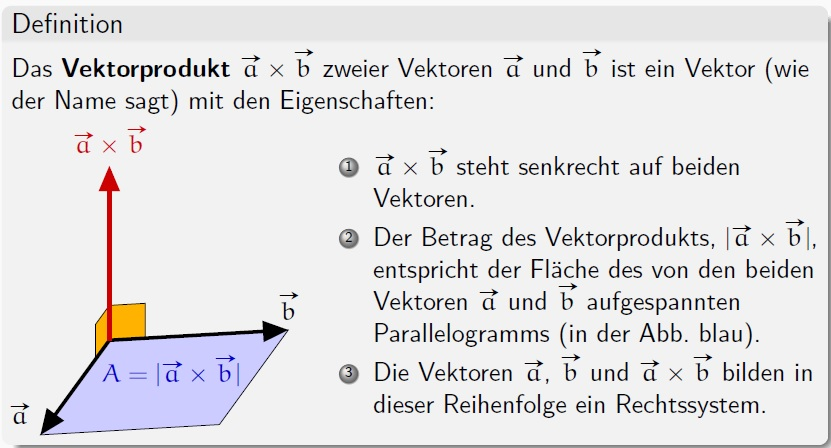
\includegraphics[width=0.7\linewidth]{fig/vektorprodukt_definition}
	\caption{Definition vom Vektorprodukt}
	\label{fig:vektorprodukt_definition}
\end{figure}

\begin{figure}[!ht]
	\centering
	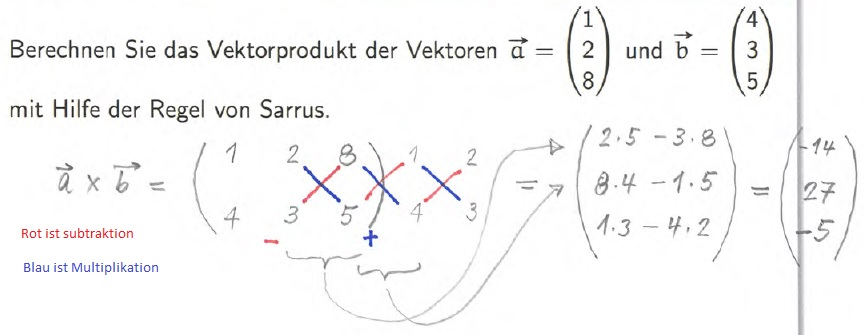
\includegraphics[width=0.7\linewidth]{fig/vektorprodukt_example1}
	\caption{Vektorprodukt Example 1}
	\label{fig:vektorprodukt_example1}
\end{figure}

\begin{figure}[!ht]
	\centering
	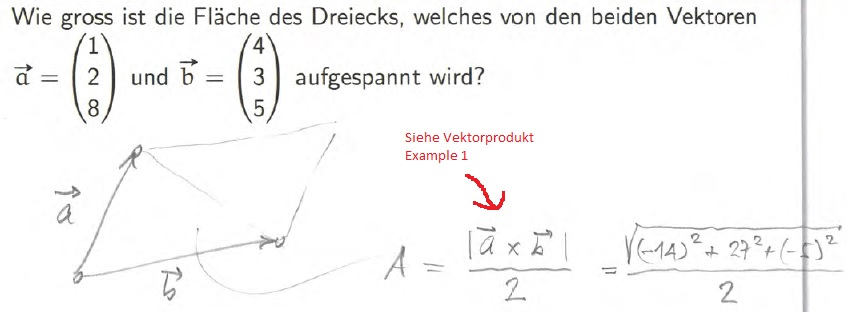
\includegraphics[width=0.7\linewidth]{fig/vektorprodukt_example2}
	\caption{Vektorprodukt Example 2}
	\label{fig:vektorprodukt_example2}
\end{figure}

\subsection{Rechenregeln für das Vektorprodukt}

\begin{math}
	\vec{a} \times \vec{b} = -\vec{b} \times \vec{a}
\end{math}
Anti-Kommutativgesetz\\
\begin{math}
	\vec{a} \times (\vec{b} + \vec{c}) = \vec{a} \times \vec{b} + \vec{a} \times \vec{c}
\end{math}
Distributivgesetz\\
\begin{math}
	\lambda (\vec{a} \times \vec{b})=
	(\lambda \vec{a}) \times \vec{b} = 
	\vec{a}  \times (\lambda \vec{b})
\end{math}

